\documentclass[sigplan,screen]{acmart}

%% \BibTeX command to typeset BibTeX logo in the docs
\AtBeginDocument{%
  \providecommand\BibTeX{{%
    \normalfont B\kern-0.5em{\scshape i\kern-0.25em b}\kern-0.8em\TeX}}}

\usepackage[ruled,vlined]{algorithm2e}

%% Rights management information.  This information is sent to you
%% when you complete the rights form.  These commands have SAMPLE
%% values in them; it is your responsibility as an author to replace
%% the commands and values with those provided to you when you
%% complete the rights form.
\setcopyright{acmcopyright}
\copyrightyear{2020}
\acmYear{2020}
\acmDOI{10.1145/1122445.1122456}

%% These commands are for a PROCEEDINGS abstract or paper.
\acmConference[PaPoC '20]{PaPoC '20: Proceedings of the 7th Workshop on Principles and Practice of Consistency for Distributed Data}{April 27, 2020}{Heraklion, Crete, Greece}
\acmBooktitle{PaPoC '20: Proceedings of the 7th Workshop on Principles and Practice of Consistency for Distributed Data,
  April 27, 2020, Heraklion, Crete, Greece}
\acmPrice{15.00}
% \acmISBN{978-1-4503-XXXX-X/18/06}


%%
%% Submission ID.
%% Use this when submitting an article to a sponsored event. You'll
%% receive a unique submission ID from the organizers
%% of the event, and this ID should be used as the parameter to this command.
%%\acmSubmissionID{123-A56-BU3}

%%
%% The majority of ACM publications use numbered citations and
%% references.  The command \citestyle{authoryear} switches to the
%% "author year" style.
%%
%% If you are preparing content for an event
%% sponsored by ACM SIGGRAPH, you must use the "author year" style of
%% citations and references.
%% Uncommenting
%% the next command will enable that style.
%%\citestyle{acmauthoryear}

%%
%% end of the preamble, start of the body of the document source.
\begin{document}

%%
%% The "title" command has an optional parameter,
%% allowing the author to define a "short title" to be used in page headers.
\title{Preserving Reciprocal Consistency in Distributed Graph Databases}

%%
%% The "author" command and its associated commands are used to define
%% the authors and their affiliations.
%% Of note is the shared affiliation of the first two authors, and the
%% "authornote" and "authornotemark" commands
%% used to denote shared contribution to the research.
\author{Paul Ezhilchelvan}
\email{paul.ezhilchelvan@ncl.ac.uk}
\orcid{0000-0002-6190-5685}
\affiliation{%
  \institution{Newcastle University}
  \city{Newcastle}
  \country{UK}
  \postcode{NE4 5TG}
}

\author{Isi Mitrani}
\email{isi.mitrani@ncl.ac.uk}
\orcid{0000-0002-7797-7755}
\affiliation{%
  \institution{Newcastle University}
  \city{Newcastle}
  \country{UK}
  \postcode{NE4 5TG}
}

\author{Jack Waudby}
\email{j.waudby2@ncl.ac.uk}
\affiliation{%
  \institution{Newcastle University}
  \city{Newcastle}
  \country{UK}
  \postcode{NE4 5TG}
}

\author{Jim Webber}
\email{jim.webber@neo4j.com}
\affiliation{%
  \institution{Neo4j}
  \streetaddress{Union House,182-194 Union Street}
  \city{London}
  \country{UK}
  \postcode{SE1 0LH}}



%%
%% By default, the full list of authors will be used in the page
%% headers. Often, this list is too long, and will overlap
%% other information printed in the page headers. This command allows
%% the author to define a more concise list
%% of authors' names for this purpose.
\renewcommand{\shortauthors}{Ezhilchelvan, et al.}

\begin{abstract}

  In this paper we formalize the notion of \textit{reciprocal consistency}, a important feature specific to graph databases. If reciprocal consistency is not enforced during transaction processing, a scale-free distributed graph database can become semantically corrupt within a short time period relative to database lifetime. Reciprocal consistency can be maintained as a part of enforcing any of several known strong isolation guarantees (e.g., snapshot isolation) incurring well established performance costs. However, in practice systems are often deployed with weaker consistency, this paper describes two protocols that provide only reciprocal consistency semantics. Catering for users that are interested only in ensuring reciprocal consistency to preserve the integrity of a distributed graph database. Both protocols presented are compared and contrasted using metrics such as number of aborts per second.


\end{abstract}

% \begin{CCSXML}
% <ccs2012>
%  <concept>
%   <concept_id>10010520.10010553.10010562</concept_id>
%   <concept_desc>Computer systems organization~Embedded systems</concept_desc>
%   <concept_significance>500</concept_significance>
%  </concept>
%  <concept>
%   <concept_id>10010520.10010575.10010755</concept_id>
%   <concept_desc>Computer systems organization~Redundancy</concept_desc>
%   <concept_significance>300</concept_significance>
%  </concept>
%  <concept>
%   <concept_id>10010520.10010553.10010554</concept_id>
%   <concept_desc>Computer systems organization~Robotics</concept_desc>
%   <concept_significance>100</concept_significance>
%  </concept>
%  <concept>
%   <concept_id>10003033.10003083.10003095</concept_id>
%   <concept_desc>Networks~Network reliability</concept_desc>
%   <concept_significance>100</concept_significance>
%  </concept>
% </ccs2012>
% \end{CCSXML}

\ccsdesc[500]{Data Management~Graph Databases}
\ccsdesc[300]{Data Management~Reciprocal Consistency}

% \ccsdesc[500]{Computer systems organization~Embedded systems}
% \ccsdesc[300]{Computer systems organization~Redundancy}
% \ccsdesc{Computer systems organization~Robotics}
% \ccsdesc[100]{Networks~Network reliability}

\keywords{Graph Databases, Reciprocal Consistency}


\maketitle

\section{Introduction}

Recent years have seen a proliferation in the use of graph technologies \cite{Besta2019}. Application areas are wide reaching from healthcare, social networks and fraud detection \cite{Eifrem2016}. Graph databases model data as a \textit{labeled property graph}, vertices represent entities and edges represent the relationship between entities; properties can be stored on both vertices and edges \cite{Robinson2015}.

In practice graphs can be extremely large \cite{Sahu2017}, exceeding the storage capacity of a single-node database. An approach to storing large graphs is to partition graph data over several machines in a cluster. Moving from a single-node database to one partitioned and distributed across servers introduces several interesting problems regarding data consistency. Graphs place a high demand on the underlying database and maintaining structural integrity across partitions - called \textit{reciprocal consistency} - in a distributed graph database is non-trivial.

In order to preserve reciprocal consistency, one could implement a heavyweight coordination protocol across partitions providing Serializability or Snapshot Isolation, which have associated performance costs. To avoid these costs database managements systems (DBMSs) provide several weak isolation models \cite{Berenson1995}. In addition, there are a number of systems that eschew transactional guarantees altogether, typically offering eventual consistency \cite{Bailis2013}. Recent work \cite{Ezhilchelvan2018} investigated how violation of reciprocal consistency can occur under eventual consistency, leading to semantic corruption at alarmingly rates. The contribution of this paper is the description of two protocols that provide only reciprocal consistency, a consistency model between the known extremes that provides suitable performance. The performance of each protocol is measured using metrics such as aborts per second.


\section{Reciprocal Consistency}
\label{sec:recipr-cons}


In the labeled property graph data model edges have direction, there is a \textit{source} and a \textit{destination} vertex. Edge information is stored with \textbf{both} the source and destination vertices. This facilitates bi-directional edge traversal and allows for better query performance.

A common approach to storing graphs (arising from JanusGraph \cite{janusgraph} and TitanDB [REF]) is for records to represent vertices containing both data values and an adjacency list containing edge ``pointers'' to other vertices. In this representation an edge has ``reciprocal'' entries in the adjacency lists of the vertices the edge connects Figure \ref{adj-list}. A query reading either the source or destination vertices should be able to reify the edge correctly, returning consistent results. When the adjacency lists for vertices are mutually compatible like this, we say they are \emph{reciprocally consistent}.

\begin{figure}[h]
  \centering
  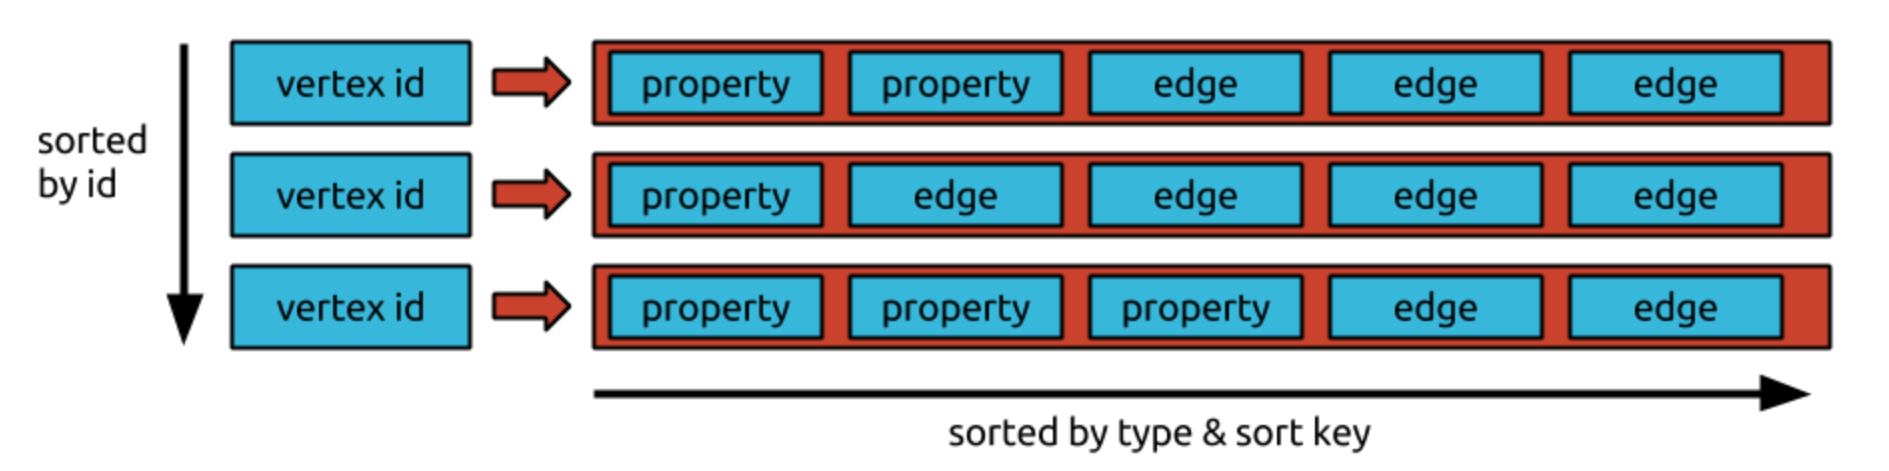
\includegraphics[width=\linewidth]{./images/janusgraph-adj-list}
  \caption{Graph representation [REF].}
  \Description{Graph representation.}
  \label{adj-list}
\end{figure}

Consider, for example, the statement that Tolkien \textit{wrote} The Hobbit. It is expressed using vertices A and B, for Tolkien and The Hobbit respectively, and an edge \textit{wrote} running from A (source) to B (destination). Adjacency lists of both A and B record information about that edge and this information is mutually reciprocal (or inverse) of each other: A's list will indicate `A \textit{wrote} B' while B's will have `B \textit{written} by A'. Thus, a query `list all titles by the author who wrote The Hobbit' can be answered by landing at B and then traversing to A; even though the edge \texttt{(A \{name:`Tolkien'\})-[:WROTE]->(B \{title:`The Hobbit'\})} is a directed edge at model level abstraction.

\section{Distributed Graph Databases}

A distributed graph database employs a shared-nothing architecture, partitioning a graph between a number of loosely cooperating servers. Graph partitioning is non-trivial and a common approach is to use a $k$-balanced edge cut \cite{Huang2016}. The objective of such an approach is to minimize the proportion of edge that span partitions in a manner that balances the distribution of vertices to partitions. Intra-partition edges are referred to as \textit{local edges} and inter-partition edges are referred to as \textit{distributed edges}, [FIG]. The proportion of distributed edges is highly data dependent. However, the number of such edges is always non-negligible ranging from 15-30\%.

\begin{figure}[h]
  \centering
  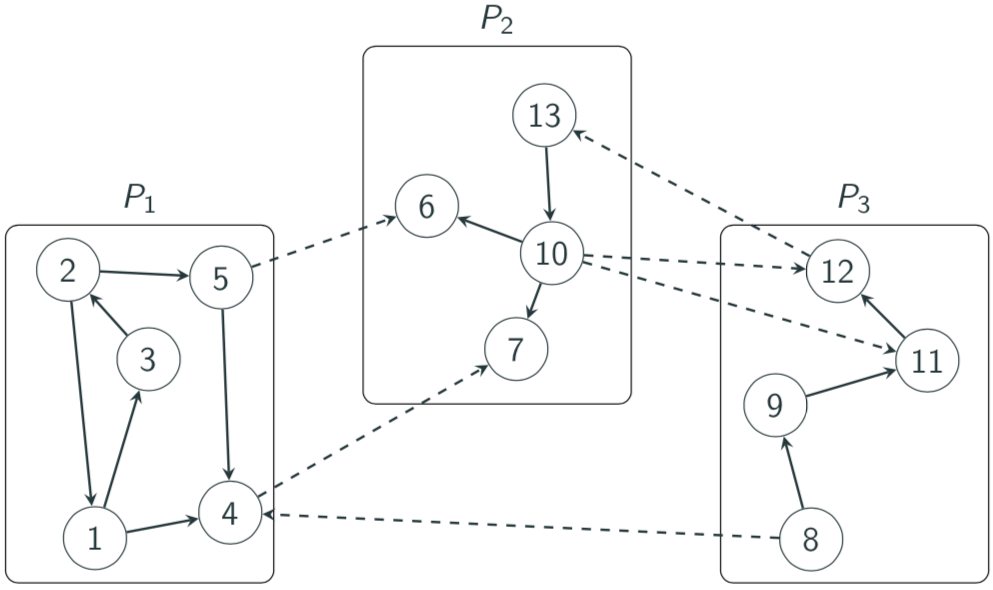
\includegraphics[width=\linewidth]{./images/dist-graph}
  \caption{A partitioned graph assigned to servers in a cluster. Some edges are local and some distributed}
  \Description{Graph representation.}
  \label{dist-graph}
\end{figure}

In a distributed graph database, adjacency lists can contain ``pointers'' to edges on remote servers. This makes maintaining distributed edge reciprocal consistency more challenging - especially given a common architecture employed by contemporary distributed graph databases. Often they use an existing eventually consistent database (e.g. Apache Cassandra [REF]) to store data, which has been adapted with a programmatic API or query language expressed in terms of edges and vertices along with some gluecode to bind that interface to the underlying database. Superficially, opting for this design appears to be a good choice: the user has the modeling convenience of graphs with the operational characteristics from the underlying database. However, the problem with this design is the (lack of) transactional semantics are inherited from the underlying store. For example, Apache Cassandra provides no way of preventing updates from mutual interference in its normal multi-partition use case. Earlier work displayed how weak isolation undermines distributed edge reciprocal consistency, causing irreversible corruption that spreads at alarmingly rates \cite{Ezhilchelvan2018}.

Of course, reciprocal consistency can be maintained as a part of enforcing any of several known strong isolation guarantees (e.g., snapshot isolation) but that incurs a performance cost if users are interested only in ensuring reciprocal consistency to preserve the integrity of a distributed database. This paper addresses that challenge.


\section{Preserving Reciprocal Consistency}


A single logical write to a distributed edge consists of two sub-operations, updating reciprocal information at the source and the destination vertices. The order in which sub-operations take place are not constrained. For example, when updating an edge between A and B it is equally likely to update A then B as it is to update B then A. Without sufficient isolation, concurrent updates can interleave in a manner that violates reciprocal consistency [FIG], such an edge is known as a \emph{half-corrupted} edge. Figure [FIG] outlines the interleavings that produce half-corrupted edges.

% transactions consists of reads/writes

\subsection{\emph{Delta} Protocol}

In order to prevent all interleaving in Figure [FIG] the \emph{Delta} protocol adopts a probabilistic approach. It is assumed there is a known $\Delta$, that reflects the bound on server communication delays, with a probability $(1-\epsilon)$ that $\Delta$ is violated. Informally, the protocol consists of two-phases. In phase 1 all writes by sub-operations are temporary and a sub-operation is allowed to proceed provided there is no other temporary sub-operation preceding it within $\Delta$; measured as per the local clock time. If the attempt does not succeed, the transaction aborts, aborting any and every previous tentative write that it may have successfully completed. In phase 2, a transaction that succeeds at all its tentative write attempts, decides to commit when it completes its graph traversal; the transaction commits once all its tentative writes are committed. This protocol avoids all conflict scenarios in Figure [FIG] provided the bound is not violated. If the bound is violate corruption and its spread can still occur, Figure [FIG]. There exists an interesting relationship between $\Delta$, the proportion of aborts and the spread of corruption.

\begin{algorithm}
  \SetAlgoLined
  \eIf{sub-operation=1}{
    \eIf{$\Delta = \emptyset$}{
      Perform tentative write operation\;
      Set $\Delta$\;
      Issue sub-operation-2\;
    }{
      Abort transaction\;
    }
  }{
    \eIf{$\Delta = \emptyset$}{
      Perform tentative write operation\;
      Set $\Delta$\;
      Continue transaction\;
    }{
      Abort transaction\;
    }
  }
    \caption{\emph{Delta} Protocol Phase 1}
\end{algorithm}

\section{Evaluation \& Results}

% Spread Corruption

\begin{figure}[h]
  \centering
  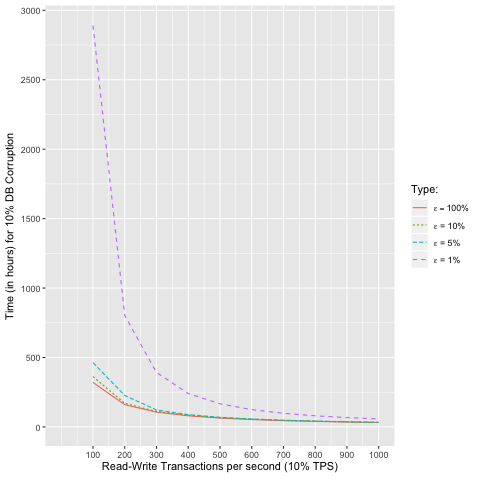
\includegraphics[width=\linewidth]{./images/corruption_comparison}
  \caption{A partitioned graph assigned to servers in a cluster. Some edges are local and some distributed}
  \Description{Graph representation.}
  \label{dist-graph}
\end{figure}

% Aborts/s

\section{Related Work}

\section{Conclusions}


% \section{Introduction}
% ACM's consolidated article template, introduced in 2017, provides a
% consistent \LaTeX\ style for use across ACM publications, and
% incorporates accessibility and metadata-extraction functionality
% necessary for future Digital Library endeavors. Numerous ACM and
% SIG-specific \LaTeX\ templates have been examined, and their unique
% features incorporated into this single new template.

% If you are new to publishing with ACM, this document is a valuable
% guide to the process of preparing your work for publication. If you
% have published with ACM before, this document provides insight and
% instruction into more recent changes to the article template.

% The ``\verb|acmart|'' document class can be used to prepare articles
% for any ACM publication --- conference or journal, and for any stage
% of publication, from review to final ``camera-ready'' copy, to the
% author's own version, with {\itshape very} few changes to the source.

% % \section{Template Overview}
% % As noted in the introduction, the ``\verb|acmart|'' document class can
% % be used to prepare many different kinds of documentation --- a
% % double-blind initial submission of a full-length technical paper, a
% % two-page SIGGRAPH Emerging Technologies abstract, a ``camera-ready''
% % journal article, a SIGCHI Extended Abstract, and more --- all by
% % selecting the appropriate {\itshape template style} and {\itshape
% %   template parameters}.

% % This document will explain the major features of the document
% % class. For further information, the {\itshape \LaTeX\ User's Guide} is
% % available from
% % \url{https://www.acm.org/publications/proceedings-template}.

% % \subsection{Template Styles}

% % The primary parameter given to the ``\verb|acmart|'' document class is
% % the {\itshape template style} which corresponds to the kind of publication
% % or SIG publishing the work. This parameter is enclosed in square
% % brackets and is a part of the {\verb|documentclass|} command:
% % \begin{verbatim}
% %   \documentclass[STYLE]{acmart}
% % \end{verbatim}

% % Journals use one of three template styles. All but three ACM journals
% % use the {\verb|acmsmall|} template style:
% % \begin{itemize}
% % \item {\verb|acmsmall|}: The default journal template style.
% % \item {\verb|acmlarge|}: Used by JOCCH and TAP.
% % \item {\verb|acmtog|}: Used by TOG.
% % \end{itemize}

% % The majority of conference proceedings documentation will use the {\verb|acmconf|} template style.
% % \begin{itemize}
% % \item {\verb|acmconf|}: The default proceedings template style.
% % \item{\verb|sigchi|}: Used for SIGCHI conference articles.
% % \item{\verb|sigchi-a|}: Used for SIGCHI ``Extended Abstract'' articles.
% % \item{\verb|sigplan|}: Used for SIGPLAN conference articles.
% % \end{itemize}

% % \subsection{Template Parameters}

% % In addition to specifying the {\itshape template style} to be used in
% % formatting your work, there are a number of {\itshape template parameters}
% % which modify some part of the applied template style. A complete list
% % of these parameters can be found in the {\itshape \LaTeX\ User's Guide.}

% % Frequently-used parameters, or combinations of parameters, include:
% % \begin{itemize}
% % \item {\verb|anonymous,review|}: Suitable for a ``double-blind''
% %   conference submission. Anonymizes the work and includes line
% %   numbers. Use with the \verb|\acmSubmissionID| command to print the
% %   submission's unique ID on each page of the work.
% % \item{\verb|authorversion|}: Produces a version of the work suitable
% %   for posting by the author.
% % \item{\verb|screen|}: Produces colored hyperlinks.
% % \end{itemize}

% % This document uses the following string as the first command in the
% % source file:
% % \begin{verbatim}
% % \documentclass[sigplan,screen]{acmart}
% % \end{verbatim}

% % \section{Modifications}

% % Modifying the template --- including but not limited to: adjusting
% % margins, typeface sizes, line spacing, paragraph and list definitions,
% % and the use of the \verb|\vspace| command to manually adjust the
% % vertical spacing between elements of your work --- is not allowed.

% % {\bfseries Your document will be returned to you for revision if
% %   modifications are discovered.}

% % \section{Typefaces}

% % The ``\verb|acmart|'' document class requires the use of the
% % ``Libertine'' typeface family. Your \TeX\ installation should include
% % this set of packages. Please do not substitute other typefaces. The
% % ``\verb|lmodern|'' and ``\verb|ltimes|'' packages should not be used,
% % as they will override the built-in typeface families.

% % \section{Title Information}

% % The title of your work should use capital letters appropriately -
% % \url{https://capitalizemytitle.com/} has useful rules for
% % capitalization. Use the {\verb|title|} command to define the title of
% % your work. If your work has a subtitle, define it with the
% % {\verb|subtitle|} command.  Do not insert line breaks in your title.

% % If your title is lengthy, you must define a short version to be used
% % in the page headers, to prevent overlapping text. The \verb|title|
% % command has a ``short title'' parameter:
% % \begin{verbatim}
% %   \title[short title]{full title}
% % \end{verbatim}

% % \section{Authors and Affiliations}

% % Each author must be defined separately for accurate metadata
% % identification. Multiple authors may share one affiliation. Authors'
% % names should not be abbreviated; use full first names wherever
% % possible. Include authors' e-mail addresses whenever possible.

% % Grouping authors' names or e-mail addresses, or providing an ``e-mail
% % alias,'' as shown below, is not acceptable:
% % \begin{verbatim}
% %   \author{Brooke Aster, David Mehldau}
% %   \email{dave,judy,steve@university.edu}
% %   \email{firstname.lastname@phillips.org}
% % \end{verbatim}

% % The \verb|authornote| and \verb|authornotemark| commands allow a note
% % to apply to multiple authors --- for example, if the first two authors
% % of an article contributed equally to the work.

% % If your author list is lengthy, you must define a shortened version of
% % the list of authors to be used in the page headers, to prevent
% % overlapping text. The following command should be placed just after
% % the last \verb|\author{}| definition:
% % \begin{verbatim}
% %   \renewcommand{\shortauthors}{McCartney, et al.}
% % \end{verbatim}
% % Omitting this command will force the use of a concatenated list of all
% % of the authors' names, which may result in overlapping text in the
% % page headers.

% % The article template's documentation, available at
% % \url{https://www.acm.org/publications/proceedings-template}, has a
% % complete explanation of these commands and tips for their effective
% % use.

% % Note that authors' addresses are mandatory for journal articles.

% % \section{Rights Information}

% % Authors of any work published by ACM will need to complete a rights
% % form. Depending on the kind of work, and the rights management choice
% % made by the author, this may be copyright transfer, permission,
% % license, or an OA (open access) agreement.

% % Regardless of the rights management choice, the author will receive a
% % copy of the completed rights form once it has been submitted. This
% % form contains \LaTeX\ commands that must be copied into the source
% % document. When the document source is compiled, these commands and
% % their parameters add formatted text to several areas of the final
% % document:
% % \begin{itemize}
% % \item the ``ACM Reference Format'' text on the first page.
% % \item the ``rights management'' text on the first page.
% % \item the conference information in the page header(s).
% % \end{itemize}

% % Rights information is unique to the work; if you are preparing several
% % works for an event, make sure to use the correct set of commands with
% % each of the works.

% % The ACM Reference Format text is required for all articles over one
% % page in length, and is optional for one-page articles (abstracts).

% % \section{CCS Concepts and User-Defined Keywords}

% % Two elements of the ``acmart'' document class provide powerful
% % taxonomic tools for you to help readers find your work in an online
% % search.

% % The ACM Computing Classification System ---
% % \url{https://www.acm.org/publications/class-2012} --- is a set of
% % classifiers and concepts that describe the computing
% % discipline. Authors can select entries from this classification
% % system, via \url{https://dl.acm.org/ccs/ccs.cfm}, and generate the
% % commands to be included in the \LaTeX\ source.

% % User-defined keywords are a comma-separated list of words and phrases
% % of the authors' choosing, providing a more flexible way of describing
% % the research being presented.

% % CCS concepts and user-defined keywords are required for for all
% % articles over two pages in length, and are optional for one- and
% % two-page articles (or abstracts).

% % \section{Sectioning Commands}

% % Your work should use standard \LaTeX\ sectioning commands:
% % \verb|section|, \verb|subsection|, \verb|subsubsection|, and
% % \verb|paragraph|. They should be numbered; do not remove the numbering
% % from the commands.

% % Simulating a sectioning command by setting the first word or words of
% % a paragraph in boldface or italicized text is {\bfseries not allowed.}

% % \section{Tables}

% % The ``\verb|acmart|'' document class includes the ``\verb|booktabs|''
% % package --- \url{https://ctan.org/pkg/booktabs} --- for preparing
% % high-quality tables.

% % Table captions are placed {\itshape above} the table.

% % Because tables cannot be split across pages, the best placement for
% % them is typically the top of the page nearest their initial cite.  To
% % ensure this proper ``floating'' placement of tables, use the
% % environment \textbf{table} to enclose the table's contents and the
% % table caption.  The contents of the table itself must go in the
% % \textbf{tabular} environment, to be aligned properly in rows and
% % columns, with the desired horizontal and vertical rules.  Again,
% % detailed instructions on \textbf{tabular} material are found in the
% % \textit{\LaTeX\ User's Guide}.

% % Immediately following this sentence is the point at which
% % Table~\ref{tab:freq} is included in the input file; compare the
% % placement of the table here with the table in the printed output of
% % this document.

% % \begin{table}
% %   \caption{Frequency of Special Characters}
% %   \label{tab:freq}
% %   \begin{tabular}{ccl}
% %     \toprule
% %     Non-English or Math&Frequency&Comments\\
% %     \midrule
% %     \O & 1 in 1,000& For Swedish names\\
% %     $\pi$ & 1 in 5& Common in math\\
% %     \$ & 4 in 5 & Used in business\\
% %     $\Psi^2_1$ & 1 in 40,000& Unexplained usage\\
% %   \bottomrule
% % \end{tabular}
% % \end{table}

% % To set a wider table, which takes up the whole width of the page's
% % live area, use the environment \textbf{table*} to enclose the table's
% % contents and the table caption.  As with a single-column table, this
% % wide table will ``float'' to a location deemed more
% % desirable. Immediately following this sentence is the point at which
% % Table~\ref{tab:commands} is included in the input file; again, it is
% % instructive to compare the placement of the table here with the table
% % in the printed output of this document.

% % \begin{table*}
% %   \caption{Some Typical Commands}
% %   \label{tab:commands}
% %   \begin{tabular}{ccl}
% %     \toprule
% %     Command &A Number & Comments\\
% %     \midrule
% %     \texttt{{\char'134}author} & 100& Author \\
% %     \texttt{{\char'134}table}& 300 & For tables\\
% %     \texttt{{\char'134}table*}& 400& For wider tables\\
% %     \bottomrule
% %   \end{tabular}
% % \end{table*}

% % \section{Math Equations}
% % You may want to display math equations in three distinct styles:
% % inline, numbered or non-numbered display.  Each of the three are
% % discussed in the next sections.

% % \subsection{Inline (In-text) Equations}
% % A formula that appears in the running text is called an inline or
% % in-text formula.  It is produced by the \textbf{math} environment,
% % which can be invoked with the usual
% % \texttt{{\char'134}begin\,\ldots{\char'134}end} construction or with
% % the short form \texttt{\$\,\ldots\$}. You can use any of the symbols
% % and structures, from $\alpha$ to $\omega$, available in
% % \LaTeX~\cite{Lamport:LaTeX}; this section will simply show a few
% % examples of in-text equations in context. Notice how this equation:
% % \begin{math}
% %   \lim_{n\rightarrow \infty}x=0
% % \end{math},
% % set here in in-line math style, looks slightly different when
% % set in display style.  (See next section).

% % \subsection{Display Equations}
% % A numbered display equation---one set off by vertical space from the
% % text and centered horizontally---is produced by the \textbf{equation}
% % environment. An unnumbered display equation is produced by the
% % \textbf{displaymath} environment.

% % Again, in either environment, you can use any of the symbols and
% % structures available in \LaTeX\@; this section will just give a couple
% % of examples of display equations in context.  First, consider the
% % equation, shown as an inline equation above:
% % \begin{equation}
% %   \lim_{n\rightarrow \infty}x=0
% % \end{equation}
% % Notice how it is formatted somewhat differently in
% % the \textbf{displaymath}
% % environment.  Now, we'll enter an unnumbered equation:
% % \begin{displaymath}
% %   \sum_{i=0}^{\infty} x + 1
% % \end{displaymath}
% % and follow it with another numbered equation:
% % \begin{equation}
% %   \sum_{i=0}^{\infty}x_i=\int_{0}^{\pi+2} f
% % \end{equation}
% % just to demonstrate \LaTeX's able handling of numbering.

% % \section{Figures}

% % The ``\verb|figure|'' environment should be used for figures. One or
% % more images can be placed within a figure. If your figure contains
% % third-party material, you must clearly identify it as such, as shown
% % in the example below.
% % \begin{figure}[h]
% %   \centering
% %   \includegraphics[width=\linewidth]{sample-franklin}
% %   \caption{1907 Franklin Model D roadster. Photograph by Harris \&
% %     Ewing, Inc. [Public domain], via Wikimedia
% %     Commons. (\url{https://goo.gl/VLCRBB}).}
% %   \Description{The 1907 Franklin Model D roadster.}
% % \end{figure}

% % Your figures should contain a caption which describes the figure to
% % the reader. Figure captions go below the figure. Your figures should
% % {\bfseries also} include a description suitable for screen readers, to
% % assist the visually-challenged to better understand your work.

% % Figure captions are placed {\itshape below} the figure.

% % \subsection{The ``Teaser Figure''}

% % A ``teaser figure'' is an image, or set of images in one figure, that
% % are placed after all author and affiliation information, and before
% % the body of the article, spanning the page. If you wish to have such a
% % figure in your article, place the command immediately before the
% % \verb|\maketitle| command:
% % \begin{verbatim}
% %   \begin{teaserfigure}
% %     \includegraphics[width=\textwidth]{sampleteaser}
% %     \caption{figure caption}
% %     \Description{figure description}
% %   \end{teaserfigure}
% % \end{verbatim}

% % \section{Citations and Bibliographies}

% % The use of \BibTeX\ for the preparation and formatting of one's
% % references is strongly recommended. Authors' names should be complete
% % --- use full first names (``Donald E. Knuth'') not initials
% % (``D. E. Knuth'') --- and the salient identifying features of a
% % reference should be included: title, year, volume, number, pages,
% % article DOI, etc.

% % The bibliography is included in your source document with these two
% % commands, placed just before the \verb|\end{document}| command:
% \begin{verbatim}
% \bibliographystyle{ACM-Reference-Format}
% \bibliography{papoc}
% \end{verbatim}
% % % where ``\verb|bibfile|'' is the name, without the ``\verb|.bib|''
% % % suffix, of t
%he \BibTeX\ file.

% % Citations and references are numbered by default. A small number of
% % ACM publications have citations and references formatted in the
% % ``author year'' style; for these exceptions, please include this
% % command in the {\bfseries preamble} (before
% % ``\verb|\begin{document}|'') of your \LaTeX\ source:
% % \begin{verbatim}
% %   \citestyle{acmauthoryear}
% % \end{verbatim}

% %   Some examples.  A paginated journal article \cite{Abril07}, an
% %   enumerated journal article \cite{Cohen07}, a reference to an entire
% %   issue \cite{JCohen96}, a monograph (whole book) \cite{Kosiur01}, a
% %   monograph/whole book in a series (see 2a in spec. document)
% %   \cite{Harel79}, a divisible-book such as an anthology or compilation
% %   \cite{Editor00} followed by the same example, however we only output
% %   the series if the volume number is given \cite{Editor00a} (so
% %   Editor00a's series should NOT be present since it has no vol. no.),
% %   a chapter in a divisible book \cite{Spector90}, a chapter in a
% %   divisible book in a series \cite{Douglass98}, a multi-volume work as
% %   book \cite{Knuth97}, an article in a proceedings (of a conference,
% %   symposium, workshop for example) (paginated proceedings article)
% %   \cite{Andler79}, a proceedings article with all possible elements
% %   \cite{Smith10}, an example of an enumerated proceedings article
% %   \cite{VanGundy07}, an informally published work \cite{Harel78}, a
% %   doctoral dissertation \cite{Clarkson85}, a master's thesis:
% %   \cite{anisi03}, an online document / world wide web resource
% %   \cite{Thornburg01, Ablamowicz07, Poker06}, a video game (Case 1)
% %   \cite{Obama08} and (Case 2) \cite{Novak03} and \cite{Lee05} and
% %   (Case 3) a patent \cite{JoeScientist001}, work accepted for
% %   publication \cite{rous08}, 'YYYYb'-test for prolific author
% %   \cite{SaeediMEJ10} and \cite{SaeediJETC10}. Other cites might
% %   contain 'duplicate' DOI and URLs (some SIAM articles)
% %   \cite{Kirschmer:2010:AEI:1958016.1958018}. Boris / Barbara Beeton:
% %   multi-volume works as books \cite{MR781536} and \cite{MR781537}. A
% %   couple of citations with DOIs:
% %   \cite{2004:ITE:1009386.1010128,Kirschmer:2010:AEI:1958016.1958018}. Online
% %   citations: \cite{TUGInstmem, Thornburg01, CTANacmart}. Artifacts:
% %   \cite{R} and \cite{UMassCitations}.

% % \section{Acknowledgments}

% % Identification of funding sources and other support, and thanks to
% % individuals and groups that assisted in the research and the
% % preparation of the work should be included in an acknowledgment
% % section, which is placed just before the reference section in your
% % document.

% % This section has a special environment:
% % \begin{verbatim}
% %   \begin{acks}
% %   ...
% %   \end{acks}
% % \end{verbatim}
% % so that the information contained therein can be more easily collected
% % during the article metadata extraction phase, and to ensure
% % consistency in the spelling of the section heading.

% % Authors should not prepare this section as a numbered or unnumbered {\verb|\section|}; please use the ``{\verb|acks|}'' environment.

% \section{Appendices}

% If your work needs an appendix, add it before the
% ``\verb|\end{document}|'' command at the conclusion of your source
% document.

% Start the appendix with the ``\verb|appendix|'' command:
% \begin{verbatim}
%   \appendix
% \end{verbatim}
% and note that in the appendix, sections are lettered, not
% numbered. This document has two appendices, demonstrating the section
% and subsection identification method.



% %%
% %% The acknowledgments section is defined using the "acks" environment
% %% (and NOT an unnumbered section). This ensures the proper
% %% identification of the section in the article metadata, and the
% %% consistent spelling of the heading.
% \begin{acks}
% To Robert, for the bagels and explaining CMYK and color spaces.
% \end{acks}

%%
%% The next two lines define the bibliography style to be used, and
%% the bibliography file.
\bibliographystyle{ACM-Reference-Format}
\bibliography{papoc}

% % %%
% % %% If your work has an appendix, this is the place to put it.
% % \appendix


\end{document}
\endinput
